%!TEX program = xelatex
% not lualatex because of a pgf bug: https://sourceforge.net/p/pgf/bugs/384/
% makeglossaries latex-version && bibtex latex-version.aux
\documentclass[12pt, a4paper]{report}
\usepackage[T1]{fontenc}
\usepackage[english]{babel}
\usepackage{hyperref}
\usepackage{utbmcovers}
\usepackage{titlesec}
\usepackage[nottoc]{tocbibind}
\usepackage{graphicx}
\usepackage{subfig}
\usepackage[acronym]{glossaries}
\usepackage{dirtytalk}
\usepackage[toc,page]{appendix}

\titleformat{\chapter}[block]{\normalfont\huge\bfseries}{\thechapter.}{5pt}{\Huge}
\titlespacing{\chapter}{0pt}{0pt}{40pt}
% \setcounter{tocdepth}{0} % Show chapters only
% \newfontfamily\italictahomafont{Tahoma}[FakeSlant=0.4]
\newfontfamily\boldtahomafont{Tahoma}[]
\graphicspath{ {images/} }
\renewcommand*{\glstextformat}[1]{\color{black}{#1}}

%----------------------------------------
% utbmcovers configuration
%----------------------------------------
\setutbmfrontillustration{report_cover}
\setutbmtitle{Deep Learning for egocentric vision}
\setutbmsubtitle{ST50 thesis - P2020}
\setutbmstudent{GUETARNI Bilel}
\setutbmstudentdepartment{Computer Science department}
\setutbmstudentpathway{Image, Interaction et Réalité Virtuelle}
\setutbmcompany{Haute Ecole d'Ingénierie et de Gestion du Canton de Vaud}
\setutbmcompanyaddress{Avenue des Sports 29\\1400 Yverdon-les-Bains}
\setutbmcompanywebsite{\href{https://heig-vd.ch/}{heig-vd.ch}}
\setutbmcompanytutor{PEREZ-URIBE Andres}
\setutbmschooltutor{GABER Jaafar}
\setutbmkeywords{Fonction publique - Recherche - Algorithmes - Logiciel d'analyse de données - Deep Learning - Computer Vision - Action recognition - Egocentric vision}
\setutbmabstract{
	Deep learning has been widely used in computer vision in the last two decades.
	Several tasks have been addressed with, including object detection, content generation, image or instance segmentation and a couple of others.
	Nowadays very complex tasks are at the heart of academic research, including action/activity recognition; these two last are really similar, the difference is slight so here we will use the term of action recognition (the difference can be for example the action of picking a fork during the activity of cooking).
	Particularly, achieving action recognition at a reasonable accuracy could allow the follow-up of people with reduced physical capacities especially with tremors in their daily life.
	It will be then easy to identify the actions that a person struggle with, and then conduct a targeted rehabilitation process.
	In this internship we explored how deep learning can be applied in action recognition and what the actual state-of-the-art is.
	We focused on cheap computation solutions as it is expected to be used on edge devices; e.g. mobile phone, embedded device\dots
}

\makeglossaries
\newglossaryentry{ego}
{
    name=egocentric view,
    description={First person view}
}
\newglossaryentry{jointly}
{
    name=jointly trained,
    description={Training several deep learning systems as one unique system}
}
\newglossaryentry{nlp}
{
    name=Natural Language Processing,
    description={Automatic process of language by computers}
}
\newglossaryentry{saliency}
{
	name=saliency,
	description={The property of an object to “stand-out” with respect to its surroundings}
}
\newglossaryentry{synthdata}
{
    name=synthetic-to-real domain gap,
    description={The unreal property of synthetic data that impacts models accuracy when trained on}
}

\begin{document}
	\makeutbmfrontcover{}

	% write table of content
	\tableofcontents{}
	
	% write acronyms
	\printglossary
	
	% set paragraph indent length
	\setlength{\parindent}{15pt}
	
	\newpage
	\chapter*{Acknowledgements}
	\addcontentsline{toc}{chapter}{\numberline{}Acknowledgements}
	I would like to express my deep gratitude to the Haute École d'Ingénierie et de Gestion du Canton de Vaud for receiving me during this internship and particulary to the International Office for providing me support, dedication and availability in these particular times.
	I would also like to thank the Communauté du Savoir that makes these extraterritorial cooperation possible that allows students to benefit from other universities education.
	Finally, I am particularly grateful to Mr. Andres PEREZ-URIBE and all his team, for all the advices, support and teaching they enthusiastically gave me.
	I adress them my very great appreciation for the assistance and the kindness they showed to me and the time they consecrated for my project.

	
	\chapter{Introduction}
		\section{Institut des Technologies de l’Information et de la Communication}
			The {\itshape Institut des Technologies de l’Information et de la Communication} (IICT) is the biggest research institute of the Haute École d'Ingénierie et de Gestion du Canton de Vaud (HEIG-VD) with more than 50 researchers and engineers and near 20 teachers.
			Its research is divided into software engineering, telecommunications, artifical intelligence, digital security and communication systems.
			They realize each year more than 60 projects, mostly with industrials.\par
			In this institut work the professor Andres PEREZ-URIBE and his team, the Intelligent Data Analysis group, on big data analysis and intelligent data analysis.
			This team \say{works on making sense of data by developing and using data-driven models using Machine Learning approaches (including artificial intelligence, artificial life and bio-inspired approaches) as an alternative to analytical models for classification, prediction, explanation and visualization}.
			They \say{aim at providing solutions to deal with the current scenario of "data deluge" (Big Data) and to provide innovative solutions for the new ubiquitous computing world (Internet of Things and Quantified Self)}.
			They developped several applications based on intelligent systems as:
			\begin{itemize}
				\item \href{http://iict.heig-vd.ch/projets#/49/agrovision-developpement-dun-outil-de-suivi-base-sur-limagerie-aerienne-a-haute-resolution-pour-une-meilleure-gestion-agronomique-et-environnementale-de-lagriculture}{Agrovision}: an aerial image based tool for agriculture monitoring.
				\item \href{http://iict.heig-vd.ch/projets#/47/clustersitg-semantic-analysis-and-clustering-of-sitg-catalogue}{ClusterSITG}: an automatic tool for metadata organization.
				\item \href{http://iict.heig-vd.ch/projets#/43/crowdstreams-analyse-et-surveillance-en-temps-r-el-de-mobilit-la-proximit-des-grands-v-nements}{CrowdStreams}: an application for crowd analyze and monitoring.
			\end{itemize}

		\section{Internship context}
			Since the availability of huge data bases, modern deep learning has been applied on several tasks with amazing performance.
			One of such tasks is action recognition.
			There have been considerable researchs on this topic using deep learning, but the lack of relatively large scaled datasets have limited the possibilities to develop supervised learning solutions.
			Rencently, there have been considerable works to create such datasets, thus, the exploration of deep learning architectures for action recognition has began.
			There is a particular dataset that concentrates on actions performed in a kitchen where the objective is to recognize a performed action (through a video) in a first person view, also called egocentric vision.
			The purpose of this internship is to create a deep learning system that is able to recognize the actions present in the dataset with the highest accuracy possible.\par
			\bigbreak
			We will first describe the relationship between deep learning and computer vision to understand which important part the first has became to the latter.
			Then, we'll review the state-of-the-art of egocentric action recognition in the literature to describe afterwards which methods were studied.
			In a critical process, we then critic the obtained results along with an interpretation.
			Finally, we'll conclude with some observations and difficulties encountered and open some roads for future investigation.

	\chapter{Action recognition in egocentric vision}
		\section{Deep Learning and Computer Vision}
			Deep Learning is a really successful field that is currently under innumerable investigations.
			Despite the well-known difficulties associated, numerous people jump into it every day.
			It has been successfully applied to several domains like Computer Vision, \gls{nlp} (NLP), board games and a raft of others.
			The first one is currently the most explored with a lot of academic research associated with huge industrial applications.
			Deep learning has revolutionized the field of computer vision by its accuracy never reached by classical algorithms.
			From the beginning, computer vision played an important role in the development of deep learning \cite{lecun_89,lecun_98,neocognitron}.
			However, it suffers from a major drawback, that is its need of enormous datasets.
			As the tasks tackled become more and more complex, the systems need more and more data to reach an acceptable accuracy.
			Also, most systems for computer vision are trained in a supervised learning fashion which requires data to be labeled, and for some tasks it is really hard to find such ones (even if synthetic data can be used, this still raise the problem of \gls{synthdata}).
			Moreover, the more data we have, the more computations are then needed, and we know that recent deep learning systems can take several weeks to train.\par
			Despite those drawbacks, and because several workarounds have been developed, deep learning is still seen as a powerful tool to enhance our systems.
			
			\subsection*{Action recognition}
			Content recognition is at the heart of the deep learning literature since the beginning. It began with numbers \cite{neocognitron,lecun_98}, animals (e.g. cats for the most popular one) and more recently complex concepts such as actions.
			Human action recognition requires developing systems that can capture motion over time (sequence prediction), or systems that can recognize an action through a single frame.
			The first case has seen emerged novels architecture as 3D convolutional networks \cite{ji} and two-stream architectures \cite{sudhakaran, wang, ye} (see \ref{twostream}).
			It is worth to notice that action recognition is itself split in two categories: first person view, also known as \gls{ego} (Figure \ref{f1}), and third person view (Figure \ref{f2}); in this work, we focus on egocentric view action recognition.
			If we look in the literature, we'll see that egocentric vision has been neglected over third person view for a long time.
			Nonetheless, large scaled recently published datasets have exposed the egocentric view problematic and encouraged research for.
			\begin{figure}[!h]
				\centering
				\subfloat[First person.]{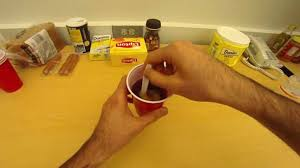
\includegraphics[width=0.4\textwidth]{firstperson.jpeg}\label{f1}}
				\hfill
				\subfloat[Third person.]{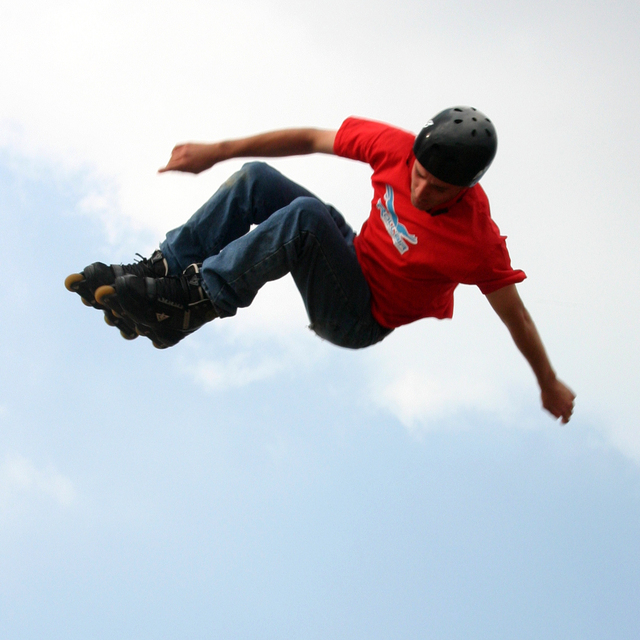
\includegraphics[width=0.4\textwidth]{thirdperson.jpg}\label{f2}}
				\caption{Action views.}
			\end{figure}
			A similar task that is increasingly covered is image captioning \cite{xu}, where a model try to add a caption to an image; which is highly related to scene understanding.
			It is easy to see that they are sensibly similar and actually, many advances that came out for image captioning are now used for action recognition (attention mechanism, recurrent neural networks).
				\subsection*{Some applications}
					Among the different applications of action recognition we find patient follow-up.
					Medical staff could use automatic egocentric action recognition to find which actions in the daily-life of a person with physical abilities disorders are the most difficult for them\footnote{Of course recognize the action is not sufficient, one should detect the disorders.}.
					And then use these analyses to conduct a targeted rehabilitation process.\par
					One should also notice the interesting potential of action recognition systems for video audio description, this could make all TV programs or videos accessible in audio description for blind or visually impaired people.
					However, it can also allow for dangerous or malicious applications as intrusive and ubiquitous surveillance.

		\section{State-of-the-art}
			In this chapter we introduce the state-of-the-art of the egocentric action recognition literature.
			We'll describe particular architecture that a majority of papers have focused on; for a particular reason.
			Furthermore, we'll see how different approaches, currently under investigation, taken from NLP have achieved considerable performance.
			
			\subsection{Two-stream architectures}\label{twostream}
				Currently, the most used architecture for action recognition is the so-called two-stream architecture.
				It consists of two subsystems, each one processing different image modalities.

				\subsubsection{Optical flows}
					As said in the introduction of this chapter, to recognize an action it is almost necessarily to capture the motion.
					This problematic of describing motion has been extremely present in the computer vision literature.
					It gave rise to optical flows, sometimes also called optical flow fields.
					An optical flow is, most of the time, computed as a shift between two gray images.
					Two types of optical flows exist: {\itshape sparse} and {\itshape dense}.
					Sparse optical flow track particular pixels among the images using feature selectors (e.g. Harris corner detector) and computes their displacment.
					On the other hand, dense optical flow is a per-pixel-motion estimate method.
					Here, we'll consider the latter one.
					% TODO: mathematical development of the two methods in appendix
					There are several methods to compute dense optical flows, but the most known (and used) are the TV-L1 \cite{sanchez} and the Gunner Farnebäck \cite{farneback} algorithms.\par
					Nowadays, even deep learning is considered for modeling optical flows (\cite{hur}).
					Note: since dense optical flow use all the pixels of 2 images, their computation is quite heavy.

				\subsubsection{Literature}
					In \cite{wang}, two Convolutional Neural Networks (CNN or ConvNet) are \gls{jointly}; rigorously speaking, one stream is trained before and used to initialize the other one before being jointly trained.
					The two-stream are identical except for the number of features expected for the input.
					The first one expect RGB images, which make 3 features, while the second one expect stacked optical flows.
					Random RGB images and optical flows are drawn from the action video and fed to their corresponding CNNs.
					At then end, a consensus function combines all the outputs to infer the final prediction.
					Notice that as the RGB images are processed individually, the motion cannot be encoded by its corresponding CNN.
					They also show that using RGB differences rather than one image improves the performances (due to the difficulty to extrapolate motion through a single frame).\par
					Yet, processing the images separately prevent the model to use the temporal correlation of the images.
					Even if we use optical flows, they describe an infinitesimal motion compared to the whole action motion.
					In \cite{ye}, this idea of using the temporal correlation of the images makes use of Recurrent Neural Networks (RNN) associated with a novel deep learning technique: ConvLSTM \cite{shi}.
					As originally developed, the Long Short-Term Memory (LSTM), that we will not present here because of its popularity, takes as input a sequence of vector and output a single vector.
					However, as we consider images it would be a waste to shrink the images into vectors for feeding them to a LSTM; because it will result in a loss of information.
					To overcome this, Shi et al. \cite{shi} developed the ConvLSTM network, that allow to process images inside a LSTM.
					For this end, they replace the matrix product by convolutions.
					This simple yet effective trick create a sort of Convolutional Recurrent Neural Network.\par
					Later on, \cite{ye} used a ResNet-101 pre-trained on ImageNet as feature extractor.
					As the others, this ConvNet is duplicate to use RGB frames and optical flows.
					The resulting feature maps of the two modes, are fused using different strategies.
					This result in a sequence of feature maps, that are fed to a ConvLSTM for temporal processing.\par
					Last but not least, a recently published paper developed a similar approach, but with an extra step.
					Sudhakaran et al. \cite{sudhakaran} pointed a major difficulty to action recognition in egocentric vision that is the \say{huge variations present in the data caused by the highly articulated nature of the human body}.
					From this, they derive an architecture that uses a widely studied mechanism nowadays, attention, that they incorporate inside a ConvLSTM.  % TODO: more informations about the architecture and its mechanisms
					They achieve the best results to this date.\par

			\subsection{EPIC-KITCHENS}
				What would be deep learning without data ?\par
				From the very beginning, people have been struggling to push deep architectures into configuration with acceptable accuracy.
				Researchers claim that the more data is gathered for training, the likeliest the model will converge.
				However, certain problems require labels that are either complex or long to create.
				For example, image segmentation requires that every pixels of an object is labeled within its category, and this, for all objects in every captured images.
				This reflects the difficulty to produce accurate and large scaled datasets for supervised learning.\par
				For egocentric action recognition, a team of researchers have published a large scaled dataset of kitchens actions in egocentric vision: \href{https://epic-kitchens.github.io/2021}{EPIC-KITCHENS}.
				This dataset has been published in 2018, \cite{damen_18}, with approximately 40K actions using more than 55 hours of recording.
				Recently, a second version came out, \cite{damen_20}, with more than 90K action segments (which have been extracted from 100 hours of recording).
				Not only it contains action recognition labels, but also action detection, action anticipation and several others challenges.
				To this date, it's the biggest open egocentric action recognition dataset available.\par
				Each action is delimited in time by is frames, and is labeled with a {\itshape verb} and a {\itshape noun} (see Figure \ref{f4}).
				\begin{figure}[!h]
					\centering
					\subfloat{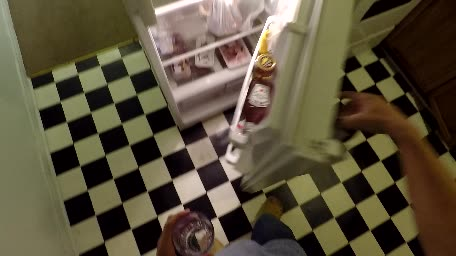
\includegraphics[width=0.55\textwidth]{close_refrigerator.jpg}\label{f4}}
					\caption{Close ({\small verb}) the refrigerator ({\small noun}).}
				\end{figure}
				The biggest advantage of using this dataset is its natural looking data.
				The videos were recording by researchers, engineers, students and other people, in their kitchens while they were doing daily stuff like: cooking, cleaning, etc.
				The resulting data has a very natural aspect which makes it suitable to train models for real world deployment.
				Note: % TODO: link to the RAM usage consideration

		\section{Studied methods}
			\subsection{Transfer Learning}
				As ConvNets architecture have become bigger and bigger over the past 20 years, the time to train these network grew exponentially.
				Therefore, people searched for a way to reduce this training time and eventually recycle the learned knowledge.
				This gave rise to Transfer Learning.
				The main argument of this practice is that big ConvNets layers, when trained on big dataset, will learn different features depending on their position in the architecture.
				Early layers tend to learn basic features such as: edge detectors, Gabor filters, etc.
				And the deeper we go in the archietecture, the more complex these features become.
				This is justified by the fact that a layer will try to detect features using combinations of the activations of its predecessor.
				Knowing this, we can assume that the early features are common features to every sort of task.
				Then we can reuse these trained models knowledge for other tasks; this is what transfer learning is all about, transfering knowledge from a domain to another.
				
			
			\subsection{LSTM and ConvLSTM}
				Lorem ipsum.
			
			\subsection{What is Attention ?}
				\say{Attention mechanism was proposed for focusing attention on features that are relevant for the task to be recognized} \cite{sudhakaran}.
				Us, humans, have the capacity to focus our {\itshape attention} into a small zone of our field of view.
				Thus, it allows us to process only the information we need and make abstraction of the rest.
				For example, while reading this, your attention is focused on these particular words and discard the surrounding ones even if they appear in your field of view.
				This way, it is easier for your mind to read.
				Attention was first used in NLP to help auto-encoders for translating long sentences (\cite{bahdanau}).
				However, the attention is used to differe
				It has then been introduced in computer vision by \cite{xu}, to help models for image captioning.
				Focusing the attention on some features requires to highlight them, so they are visually more interesting.
				In computer vision this can be seen as \gls{saliency} (Figure \ref{f3}).
				\begin{figure}[!h]
					\centering
					\subfloat{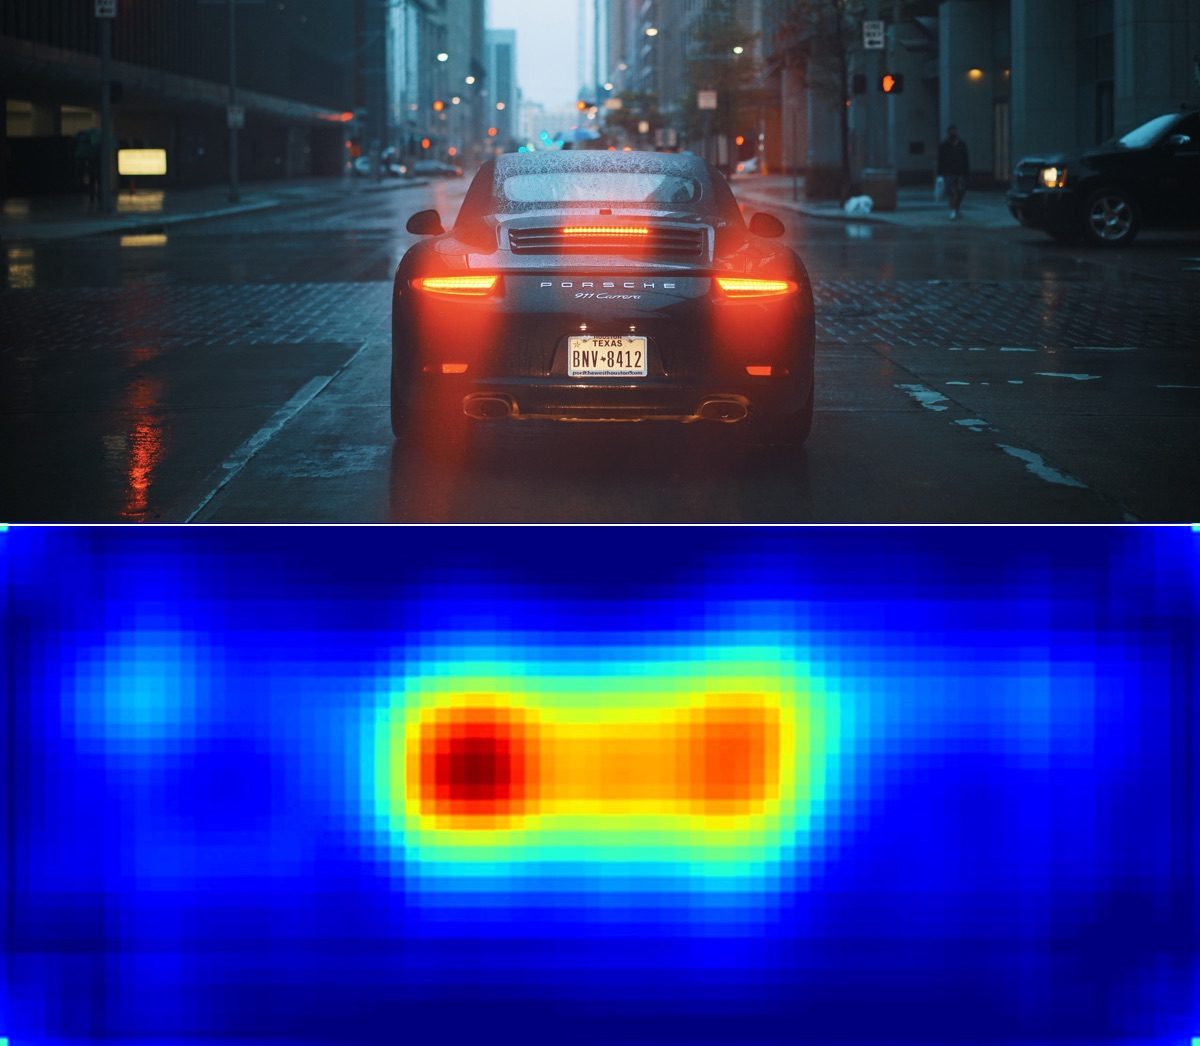
\includegraphics[width=0.4\textwidth]{porsche-saliency.jpeg}\label{f3}}
					\caption{Saliency map of a car as seen by a human.}
				\end{figure}
				In deep learning, one could use weights to make some features more visible than others.
				In \cite{sudhakaran_lanz}, the features maps extracted by a pre-trained backbone are used as weights to encode visual attention in RGB frames; rigorously speaking, the weights are derived from a pre-classification of these features maps.
				Then these weighted frames go through a ConvLSTM for classification.
				These weighted frames are called {\itshape Spatial Attention Map}.
	
		\section{Results and interpretation}
			Lorem ipsum.

		\section{Tools}
			Lorem ipsum.

	\chapter{Conclusion}
		\section{Results synthesis}
			Lorem ipsum.
		
		\section{Observations}
			Lorem ipsum.
		
		\section{Difficulties and problems}
			Lorem ipsum.
		
		\section{Roads for investigation}
			Lorem ipsum.
		
		\section{Acquired knowledge and skills}
			Lorem ipsum.
	
	\bibliographystyle{unsrt}
	\bibliography{bibliography}
	
	\appendix
	\chapter{Appendix A}
		Lorem ipsum.

	\chapter{Appendix B}
		Lorem ipsum.

	\makeutbmbackcover{}
\end{document}
